\documentclass[8pt]{report}
\usepackage{amsmath, xfrac, enumitem, graphicx, ulem, float, bigints, bm, textcomp}
\usepackage{titlesec, mathtools}
\usepackage[margin=0.7in]{geometry}
\graphicspath{ {images/} }
\linespread{0.8}
\title{\Huge{\textsc{Engineering Mechanics - GATE}}}
\author{\huge{\textbf{Kulasekaran}}}
\begin{document}
\maketitle
\tableofcontents
%-----------------------------------------------------------------------------------------%
\chapter{Composition, Resolution and Equilibrium of Forces}
\section{Force}
	\begin{itemize}
		\item It is the action of one body on another that changes the state of being (rest/uniform motion) of the object on which it is being applied
		\item 3 things are needed to define a force: Magnitude, direction, Point of application
		\item According to Newton's first law: $\boxed{Force = Mass\;*\;Acceleration}$
	\end{itemize}\hrulefill
\section{Force systems}
	\begin{itemize}
		\item \textbf{Coplanar} - 2D system
		\item \textbf{Non-Coplanar} - 3D system
	\end{itemize}
	\subsection{Collinear}
		\begin{itemize}
			\item Two are more forces whose line of action is same
			\begin{figure}[H]
				\centering
				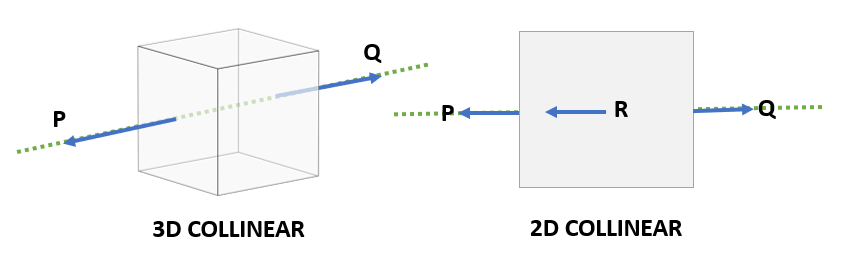
\includegraphics[scale=0.5]{collinear.png}
			\end{figure}
		\end{itemize}
	\subsection{Concurrent}
		\begin{itemize}
			\item Two are more forces which meet at a common point
			\begin{figure}[H]
				\centering
				\includegraphics[scale=0.2]{3dconcurrent.png}
				\includegraphics[scale=0.4]{2dconcurrent.png}
			\end{figure}
		\end{itemize}
	\subsection{Coplanar}
		\begin{itemize}
			\item Forces that are on the same plane
		\end{itemize}
	\subsection{Coplanar Concurrent}
		\begin{itemize}
			\item Forces that are on the same plane and meet at a common point as well
		\end{itemize}
	\subsection{Non-Coplanar Concurrent}
		\begin{itemize}
			\item Forces are not on the same plane but meet at a common point
		\end{itemize}
	\subsection{Coplanar Non-Concurrent}
		\begin{itemize}
			\item Forces are on the same plane but don't meet at a common point
		\end{itemize}
	\subsection{Non-Coplanar Non-Concurrent}			
		\begin{itemize}
			\item Forces are neither on the same plane nor meet at a common point
		\end{itemize}\hrulefill
%-----------------------------------------------------------------------------------------%
\section{Triangular Law of forces}
	\begin{itemize}
		\begin{figure}[H]
			\centering
			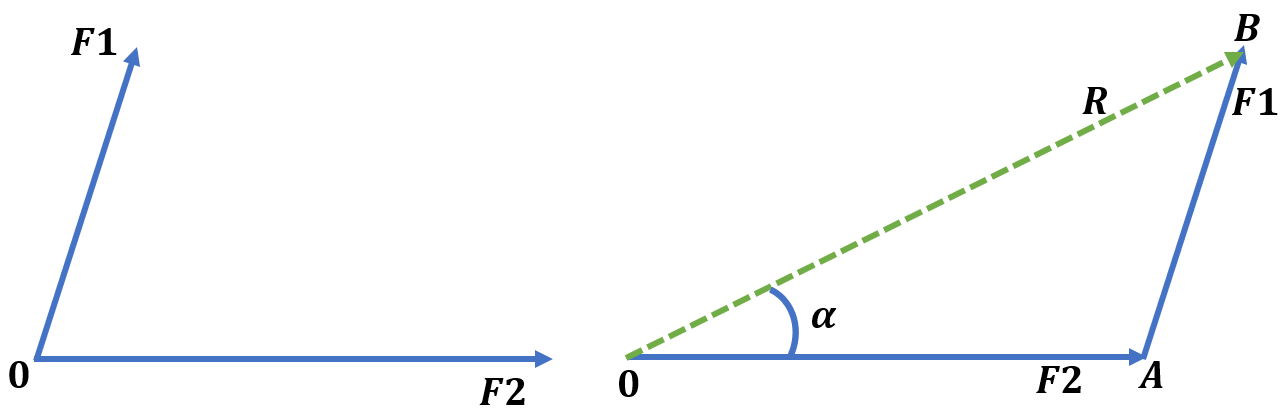
\includegraphics[scale=0.4]{triangularlaw.png}
		\end{figure}
		\item \textit{Two concurrent forces acting on a body is represented in magnitude and direction by two sides of a triangle taken in order, then their third side will represent the resultant of two forces in the direction and magnitude taken in opposite order}
		\item[] $$\boxed{R=\sqrt{F_1^2+F_2^2}}\;\;\boxed{\alpha=\cos^{-1}\left(\dfrac{F_1}{R}\right) = \sin^{-1}\left(\dfrac{F_2}{R}\right)}$$
	\end{itemize}\hrulefill		
%-----------------------------------------------------------------------------------------%
\section{Parallelogram Law of forces}
	\begin{itemize}
		\item \textit{If two concurrent forces are represented in magnitude as the two sides of a parallelogram, then the resultant of these two forces is the diagonal of the parallelogram}
		\begin{figure}[H]
			\centering
			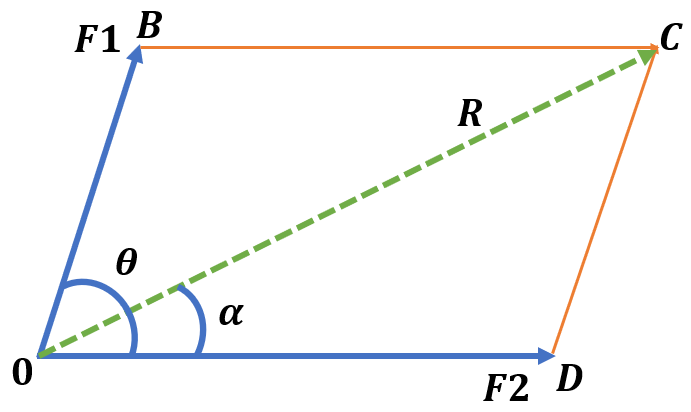
\includegraphics[scale=0.4]{parallelogramlaw.png}
		\end{figure}
		\item[] $$\boxed{R = \sqrt{F_1^2+2F_1F_2\cos\theta+F_2^2}}$$
	\end{itemize}\hrulefill
%-----------------------------------------------------------------------------------------%
\section{Polygon Law of forces}
	\begin{itemize}
		\begin{figure}[H]
			\centering
			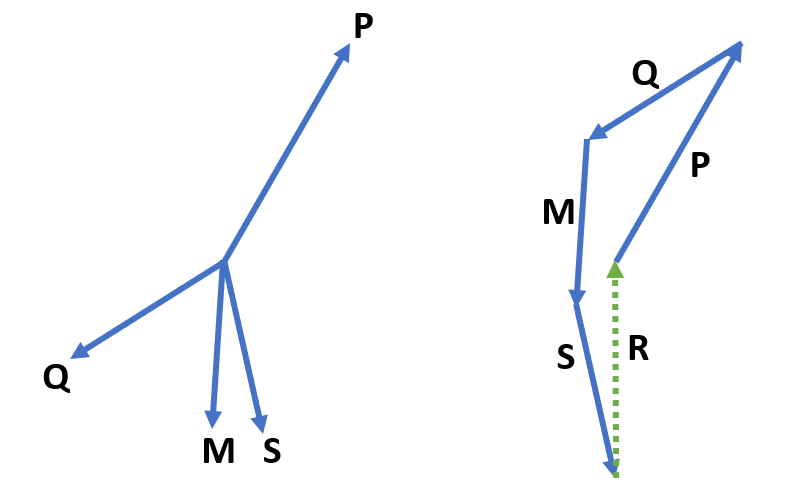
\includegraphics[scale=0.4]{polygonlaw.png}
		\end{figure}
		\item The triangular law can be extended to the polygon law. \textit{If a number of coplanar concurrent forces are represented in magnitude and direction by the sides of a polygon, taken in order, then their resultant can be represented by the closing side of the polygon}
	\end{itemize}\hrulefill
%-----------------------------------------------------------------------------------------%
\section{Resolution of Forces}
	\begin{itemize}
		\item The concept of replacing a single force at some angle with two of its component in the vertical and horizontal direction is called Resolution of forces.
		\begin{figure}[H]
			\centering
			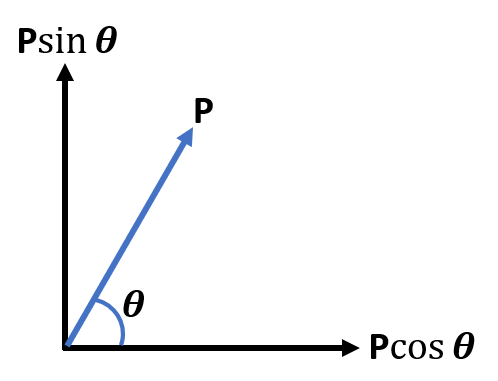
\includegraphics[scale=0.4]{resolution.png}
		\end{figure}
	\end{itemize}\hrulefill		
%-----------------------------------------------------------------------------------------%
\section{Equilibrium state}
	\begin{itemize}
		\item A body is said to be in equilibrium if it is at rest or moving with uniform velocity. \textbf{Under equilibrium state, the resultant of the force system will be zero.} 
	\end{itemize}\hrulefill
%-----------------------------------------------------------------------------------------%
\section{Lami's Theorem}
	\begin{table}[H]
		\begin{tabular}{cc}
			\parbox{4cm}{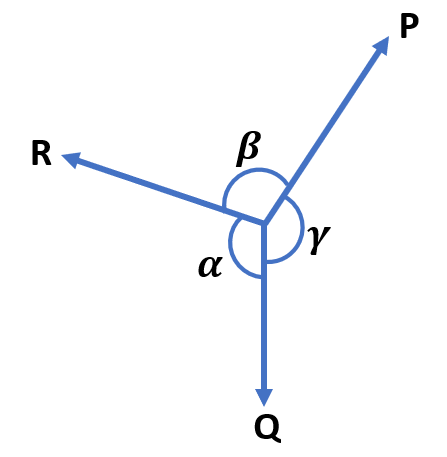
\includegraphics[scale=0.4]{lamistheorem}} &
			\parbox{12cm}{\textit{If 3 coplanar concurrent forces are in equilibrium, then each force is proportional to the sine of the angle between the other two sides}\\$$\boxed{\dfrac{P}{\sin\alpha}=\dfrac{Q}{\sin\beta}=\dfrac{R}{\sin\gamma}}$$}
		\end{tabular}			
	\end{table}\hrulefill
%-----------------------------------------------------------------------------------------%
\chapter{Analysis of Simple trusses}
\section{Plane Trusses}
	\begin{itemize}
		\item Plane Trusses - 2D trusses - All members lie on the same plane
		\item Designed to resist Geometrical distortion under loading
		\item Usually slender - CS Area very less compared to length
		\item \textbf{Two force members} - Theoretically carry only axial forces, Either in tension or in compression
	\end{itemize}\hrulefill
%-----------------------------------------------------------------------------------------%
\subsection{Perfect Trusses}
	\begin{itemize}
		\item Truss with just the right amount of members to avoid any distortion under loading
		\item Simplest perfect truss = Triangle
		\item \fbox{\textbf{Maxwell's Truss equation}: $m = 2j-3 \impliedby$ (m=No. of member, j = No. of joints)}
		\begin{itemize}
			\item Perfect truss $\implies m = 2j-3$ (Do not change in shape, right no of members)
			\item Imperfect truss $\implies m < 2j-3$ (change in shape, deficient members)
			\item Redundant truss $\implies m > 2j-3$ (Do not change in shape, extra members)
		\end{itemize}
	\end{itemize}\hrulefill
%-----------------------------------------------------------------------------------------%
\section{Types of Supports}
\subsection{Roller support}
	\begin{itemize}
		\item They are frictionless and provide only one reaction component that is vertical to its base
	\end{itemize}\hrulefill
%-----------------------------------------------------------------------------------------%
\subsection{Hinged support}
	\begin{itemize}
		\item They are fixed to their base and provide both horizontal and vertical reaction forces
	\end{itemize}\hrulefill
%-----------------------------------------------------------------------------------------%
\section{Truss Analysis}
	\begin{itemize}
		\item Involves finding support reactions and force in members
		\item Assumptions:
			\begin{itemize}
				\item Members are \textbf{Rigid} and lie in one plane (in case of plane truss)
				\item Members are \textbf{slender, Uniform cross-section}
				\item Members are subjected to pure axial force and cannot develop moments at ends
				\item External loads and reactions act at the joints only
				\item Self weight of the members is negligible
				\item Forces are transmitted from one member to another via frictionless pins connecting the members
			\end{itemize}
		\item Methods to Analyse Trusses
			\begin{itemize}
				\item Method of Joints
				\item Method of Sections
			\end{itemize}
		\item Mostly questions in this topic is focused on:
			\begin{itemize}
				\item \textbf{Zero force member} - Member that is not under any force
				\item whether a member is under tension or compression
			\end{itemize}
	\end{itemize}\hrulefill
%-----------------------------------------------------------------------------------------%
\subsection{Method of Joints}
	\begin{itemize}
		\item In this method, $\sum F_x and \sum F_y$ for any joint, must be equal to Zero. (Static equilibrium)
		\item FBD of entire truss is drawn and the support reactions are found first using $\sum F_x = 0, \sum F_y=0, \sum M=0$
		\item Then start from a joint where there are not more than 2 unknown forces. Assume the direction of the forces of the members and in the end if they come out to be positive, then the assumed direction is right, else, the assumed direction is wrong.
		\item If a member pulls the joint to which it is connected, then it is subjected to Tensile force.
		\item If a member pushes the joint to which it is connected, then it is subjected to compressive force.
		\item \textbf{Tie} - Member under Tension, \textbf{Strut} - Member under Compression
	\end{itemize}\hrulefill
%-----------------------------------------------------------------------------------------%
\subsection{Method of Sections}
	\begin{itemize}
		\item The truss is split into 2 parts by an imaginary section
		\item The section must not cut through more than 3 members with unknown forces
		\item The equilibrium conditions are applied for one part and the unknown forces in that part are determined
		\item Similar to the Method of joints, here also, at first the forces are assumed directions and based on its outcome its verified/changed
	\end{itemize}\hrulefill
%-----------------------------------------------------------------------------------------%
\subsection{Tricks for finding Zero Force Member}
	\begin{itemize}
		\item If at a an unloaded joint (a joint with no external load) with three members, two collinear forces are acting, then the third member will be a Zero Force member	
		\item In the below shown example, in Left figure, Member \textbf{DC, EF, HG} are Zero force members and in the right figure, Member \textbf{AC, CD} are Zero force members	
		\begin{figure}[H]
			\centering
			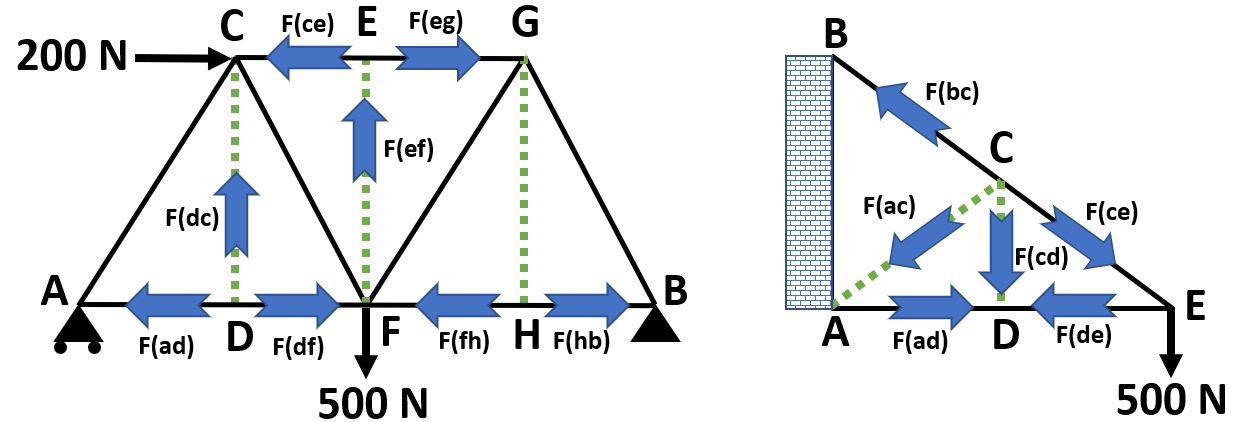
\includegraphics[scale=0.5]{zeroforcemember.png}
		\end{figure}
	\end{itemize}\hrulefill
%-----------------------------------------------------------------------------------------%
\chapter{Friction}
\section{Introduction}
	\begin{itemize}
		\item When two bodies are in contact and when one body is moved with respect to another, there develops a tangential force between the bodies trying to prevent motion. 
		\item Friction always develops opposite to the direction of motion
		\item The rougher the surface, more will be the friction
		\item Only when applied force is higher than the frictional force, there will be motion
	\end{itemize}
\subsection{Dry Friction}
	\begin{itemize}
		\item Friction between two Non-lubricated solids with motion or tendency of motion
	\end{itemize}
\subsection{Fluid Friction}
	\begin{itemize}
		\item Friction between two layers of liquid in a flow. Also known as \textbf{Viscosity}. Dealt with in Fluid Mechanics
	\end{itemize}
\subsection{Static Friction and Static Friction laws}
	\begin{itemize}
		\item When applied force is less than the frictional force and so the body is not set in motion, that frictional force is called Static friction
		\item[$\implies$] Limiting frictional force $\propto$ Normal reaction between two contact surfaces
		\item[$\implies$] \textbf{Friction is independent of area of contact/shape}
	\end{itemize}
\subsection{Dynamic Friction}
	\begin{itemize}
		\item If the body was set in motion due to applied force being higher than the frictional force between them, then that frictional force still being experience by the moving body is called dynamic friction
	\end{itemize}
%-----------------------------------------------------------------------------------------%
\section{Coefficient of Friction}
	\begin{itemize}
		\item We know $Limiting\;friction\;\propto\;Normal\;Force \implies \boxed{F_{SL} = \mu_{SF} N}\impliedby (\mu_{SF}$ = Coefficient of static friction)
		\item $\boxed{F_{DL}=\mu_{DF}N}\impliedby(\mu_{DF}$ = Coefficient of Dynamic friction)
		\item $\boxed{\mu_{SF}>\mu_{DF}}\impliedby$ as ($F_{SL}>F_{DL}$) $\impliedby F_{SL}$ = Static Limiting friction, $F_{DL}$ = Dynamic Limiting friction
	\end{itemize}\hrulefill
%-----------------------------------------------------------------------------------------%
\section{Angle of Friction ($\phi$)}
	\begin{itemize}
		\begin{figure}[H]
			\centering
			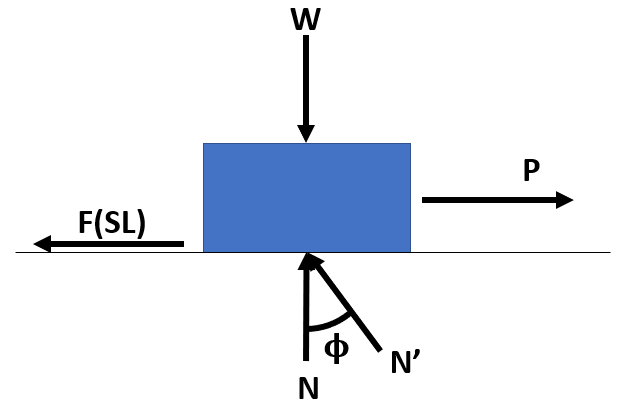
\includegraphics[scale=0.5]{angleoffriction.png}
		\end{figure}
		\item It is the angle between the resultant($N'$) of limiting friction($F_{SL}$) and Normal force($N$) and the Normal force($N$). $\boxed{N' = \sqrt{N^2+F_{SL}^2}}$
		\item $\boxed{\tan\phi=\dfrac{F_{SL}}{N}}\implies \tan\phi=\mu_{SF}\implies\boxed{\phi=\tan^{-1}(\mu_{SF})}$
	\end{itemize}\hrulefill
%-----------------------------------------------------------------------------------------%
\section{Angle of repose ($\alpha$)}
	\begin{itemize}
		\item The max angle of plane inclination for which a body resting on such plane will not slide due to its own weight is called \textbf{Angle of Repose}
		\begin{figure}[H]
			\centering
			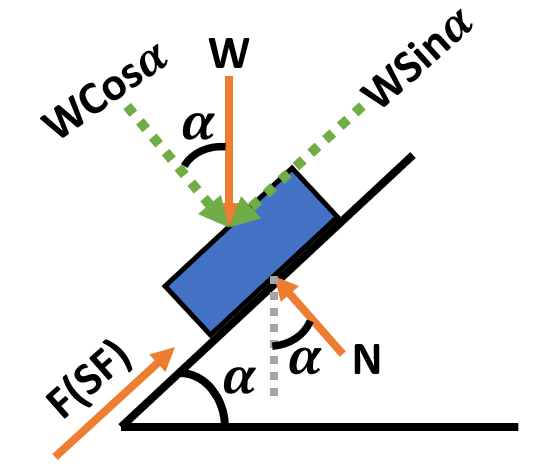
\includegraphics[scale=0.5]{angleofrepose.png}
		\end{figure}
		\item $W\cos\alpha=N$ and $W\sin\alpha=F_{SF}\implies W\sin\alpha=\mu_{SF}N$
		\item Dividing the above will give us $\tan\alpha=\mu_{SF}$ But $\mu_{SF}=\tan\phi$
		\item So, it can be stated that \fbox{\textbf{Angle of repose = Angle of friction}}
	\end{itemize}\hrulefill	
%-----------------------------------------------------------------------------------------%
\section{Wedge}
\subsection{Load(W)}
	\begin{itemize}
		\item  Weight lifted (or) resistance overcome by the machine
	\end{itemize}
\subsection{Effort(P)}
	\begin{itemize}
		\item Force required by the machine to lift the load $\boxed{P = W\tan(2\phi+\alpha)}$
	\end{itemize}
\subsection{Mechanical Advantage}
	\begin{itemize}
		\item $\boxed{MA = \dfrac{W}{P}}$
		\item Changes wrt to changes in friction
		\item Some machines have MA less than 1 $\implies$ They require more effort than load lifted.
		\item For a wedge, if $\alpha\downarrow$, then $MA\uparrow$ 
		\item MA for both single and double wedge is same for same $\alpha$
	\end{itemize}
\subsection{Input}
	\begin{itemize}
		\item Work done by effort(P) $\implies$ (P * Distance of movement = P * x)
	\end{itemize}
\subsection{Output}
	\begin{itemize}
		\item Work done by machine $\implies$ (W * Distance of movement = W * y)
	\end{itemize}
\subsection{Efficiency($\eta$)}
	\begin{itemize}
		\item $\boxed{\eta=\dfrac{Output}{Input} = \dfrac{W*y}{P*x} = \dfrac{MA}{VR}}$
		\item As Efficiency for a machine is always less than one, this implies \textbf{MA is always less than VR}
	\end{itemize}
\subsection{Velocity ratio(VR)}
	\begin{itemize}
		\item $\boxed{VR = \dfrac{Velocity\;of\;effort}{Velocity\;of\;load} = \dfrac{x/t}{y/t} = \dfrac{x}{y}}$
		\item Depends only on geometrical features of the machine
		\item Constant for a machine
		\item For a wedge, $\boxed{VR = \dfrac{L}{W}} = Slope^{-1} \impliedby$ (L = length, W = Width)
		\item VR is different for single wedge and double wedge with same $\alpha$
	\end{itemize}\hrulefill
%-----------------------------------------------------------------------------------------%
\section{Rolling friction}
	\begin{table}[H]
		\begin{tabular}{cc}
			\parbox{4cm}{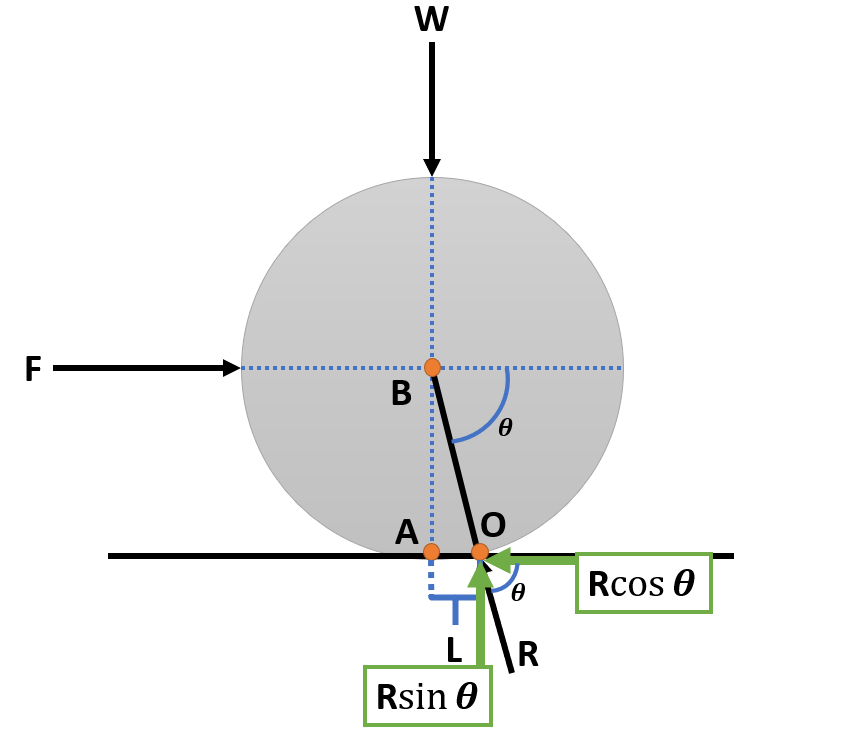
\includegraphics[scale=0.4]{rollingfriction.png}} & \hspace{2cm}
			\parbox{12cm}{Consider a wheel of radius r and Weight(W) \\\\ Taking moment about O, we get $F.r = W.L$ and by $\sum F_x=0 \implies F = R\cos\theta$ \\\\ \textbf{Rolling resistance} = $R\cos\theta$ \\\\ \textbf{Coefficient of Rolling resistance = L}\\\\ It may be noted that rolling motion is caused by a couple of applied force and rolling resistance\\\\Rolling friction always greater than Sliding friction}
		\end{tabular}
	\end{table}\hrulefill
%-----------------------------------------------------------------------------------------%
\section{Motion of a cyclist on a circular level road}
	\begin{table}[H]
		\centering
		\begin{tabular}{cc}
			\parbox{9cm}{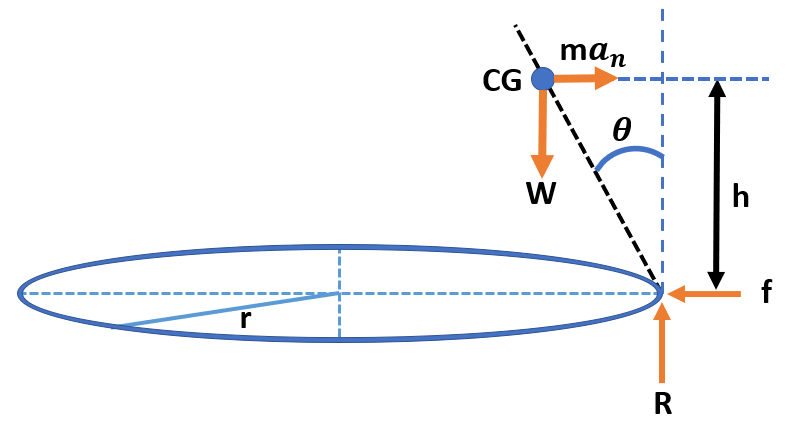
\includegraphics[scale=0.5]{cyclist_circular.png}} & 
			\parbox{12cm}{$\rightarrow$ Cyclist of weight (W) and mass (m)\\\\$\rightarrow$ moving on a circular path with radius (r)\\\\$\rightarrow$ at a constant velocity (v)\\\\$\rightarrow$ distance between CG of the cyclist and ground = h\\\\$\rightarrow$ Angle of leaning with respect to vertical = $\theta$}
		\end{tabular}
	\end{table}
	\subsection{Angle of Leaning($\theta$)}
		\begin{itemize}
			\item Centripetal acceleration developed would be : $a_n = \dfrac{V^2}{r}$
			\item The cyclist has to lean inward to maintain dynamic equilibrium and an inertial force $ma_n$ is acting on the cyclist
			\item By applying $\sum M=0$ about the point of contact, we get: $W(h\tan\theta)-(ma_n)h=0 \implies \boxed{\theta=\tan^{-1}\left(\dfrac{V^2}{rg}\right)}$ 
		\end{itemize}
	\subsection{Maximum speed ($v_{max}$) to avoid skidding}
		\begin{itemize}
			\item By $\sum F_y = 0 \implies R = W$ and $\sum F_x=0 \implies ma_n=f$
			\item Skidding is avoided if the frictional force(f) is greater than or equal to centrifugal force
			\item $\implies f_{max} = \mu R = \mu W$
			\item So, to avoid skidding : $\mu W \geq \dfrac{W}{g}\left(\dfrac{V^2}{r}\right) \implies \boxed{V_{max}\le\sqrt{\mu gr}}$
		\end{itemize}\hrulefill
%-----------------------------------------------------------------------------------------%
\section{Motion of 4-Wheeler on a circular road}
	\begin{table}[H]
		\begin{tabular}{cc}
			\parbox{4cm}{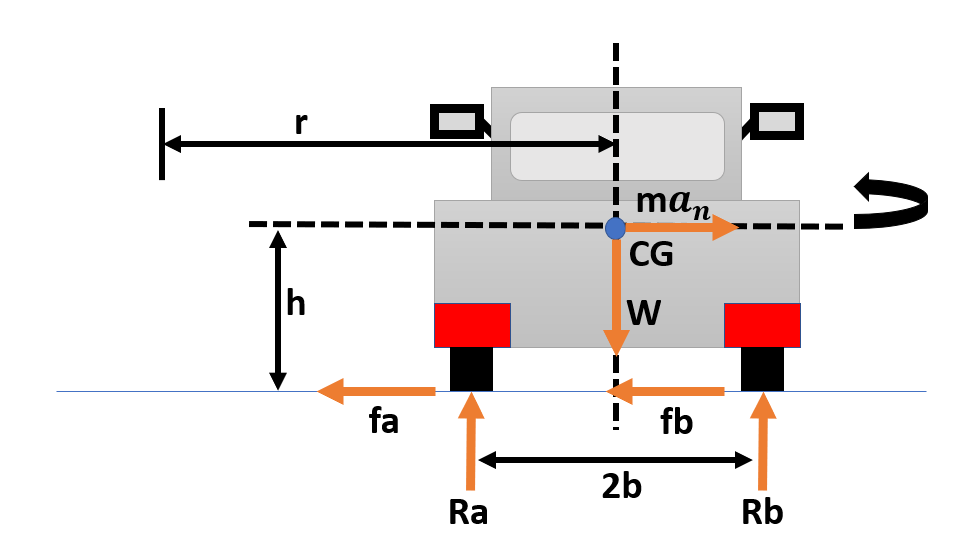
\includegraphics[scale=0.5]{4wheeler_circular.png}} & \hspace{5.8cm}
			\parbox{12cm}{$\rightarrow$ Consider a 4 wheeled vehicle with Weight(w)\\\\$\rightarrow$ Moving with uniform velocity(v)\\\\$\rightarrow$ Center of Gravity at height(h) from ground\\\\$\rightarrow$ Distance between wheels (2b)}
		\end{tabular}
	\end{table}
	\subsection{Reaction forces}
		\begin{itemize}
			\item By $\sum F_y=0$, we get $R_A + R_B = W$ (By symmetry itself we can say that $R_A$ will be equal to $R_B$)
			\item By applying $\sum M_A=0$, we get $Wb+ma_nh=2bR_B \implies Wb+\left(\dfrac{W}{g}\right)\left(\dfrac{V^2}{r}\right)h=2bR_B$
			\item So, $R_B=\dfrac{Wb}{2b}+\left(\dfrac{WV^2h}{2bgr}\right) \implies \boxed{R_B=\dfrac{W}{2}\left(1+\dfrac{V^2h}{bgr}\right)}$
			\item So, $R_A = W-R_B = W-\dfrac{W}{2}\left(1+\dfrac{V^2h}{bgr}\right) \boxed{R_A=\dfrac{W}{2}\left(1+\dfrac{V^2h}{bgr}\right)} $
		\end{itemize}
	\subsection{Max Speed to avoid Overturning}
		\begin{itemize}
			\item Overturning = Side wheeling = Only outward wheels touching the ground
			\item To find the speed limit of Overturning, we can equate the inward wheel reaction to zero, in this case $R_A\geq 0 \implies \dfrac{W}{2}\left(1+\dfrac{V^2h}{bgr}\right)\geq 0 \implies \boxed{ \dfrac{V^2h}{bgr}\geq 1}$
		\end{itemize}
	\subsection{Max Speed to avoid skidding}
		\begin{itemize}
			\item To avoid skidding $\left(ma_n\le f_a + f_b\right) \implies \dfrac{WV^2}{gr}\le\mu(R_A+R_B) \implies \dfrac{WV^2}{gr}\le \mu W \implies \boxed{V_{max} = \sqrt{\mu gr}}$
		\end{itemize}\hrulefill
%-----------------------------------------------------------------------------------------%
\section{Motion of 4-wheeler on Banked circular path}
	\begin{table}[H]
		\begin{tabular}{cc}
			\parbox{4cm}{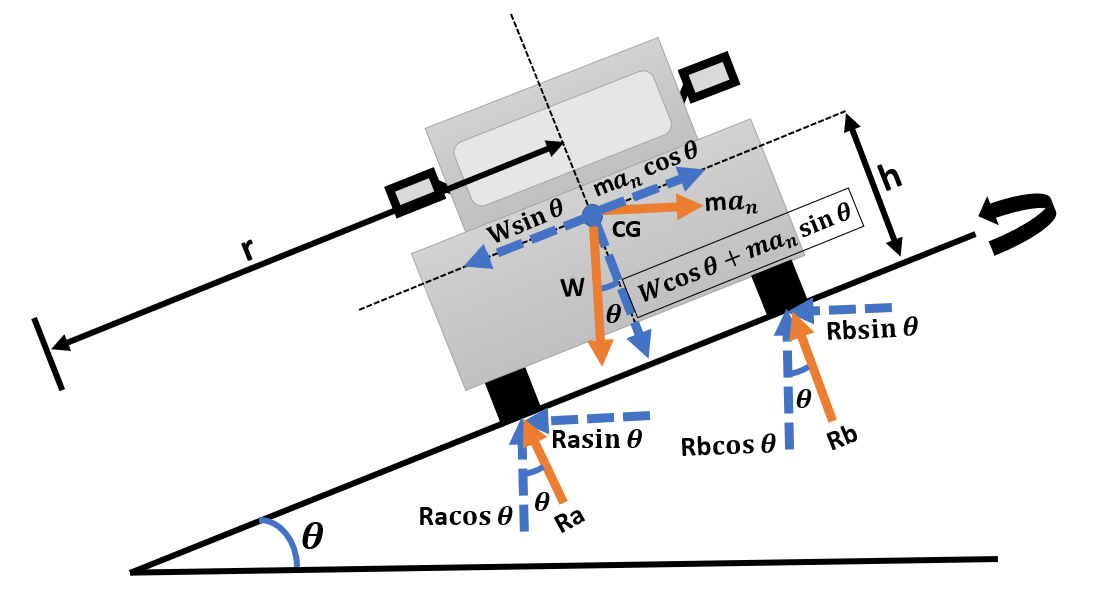
\includegraphics[scale=0.45]{vehiclebanked.png}} & \hspace{6.5cm}
			\parbox{12cm}{$\rightarrow$ Consider a Vehicle with weight(W)\\\\$\rightarrow$ Moving with a Optimum velocity(v)\\\\$\rightarrow$ On a banked circular path with slope($\theta$)\\\\}
		\end{tabular}
	\end{table}
	\subsection{Optimum speed to negotiate curved path}
	\begin{itemize}
		\item By $\sum F_x=0$ we get, $ma_n=(R_a+R_b)\sin\theta \implies \dfrac{WV^2}{gr}=(R_a+R_b)\sin\theta$
		\item By $\sum F_y=0$ we get, $W=(R_a+R_b)\cos\theta$
		\item By dividing the above two equations, we obtain: $\tan\theta=\dfrac{V^2}{gr} \implies \boxed{V=\sqrt{gr\tan\theta}} \impliedby$ (Optimum speed to negotiate curved path)
		\item If the speed of the vehicle is below the Optimum speed, then due to gravity, the vehicle will tend to fall inwards and so the tyres will experience outward frictional force
		\item \textbf{If the speed of the vehicle is equal to Optimum speed, then the tyres won't experience lateral frictional force}
		\item If the speed of the vehicle is above the Optimum speed, then the tyres will experience inward frictional force
	\end{itemize}\hrulefill
%-----------------------------------------------------------------------------------------%
\section{Motion of Locomotive on a Banked circular path}
	\begin{figure}[H]
		\centering
		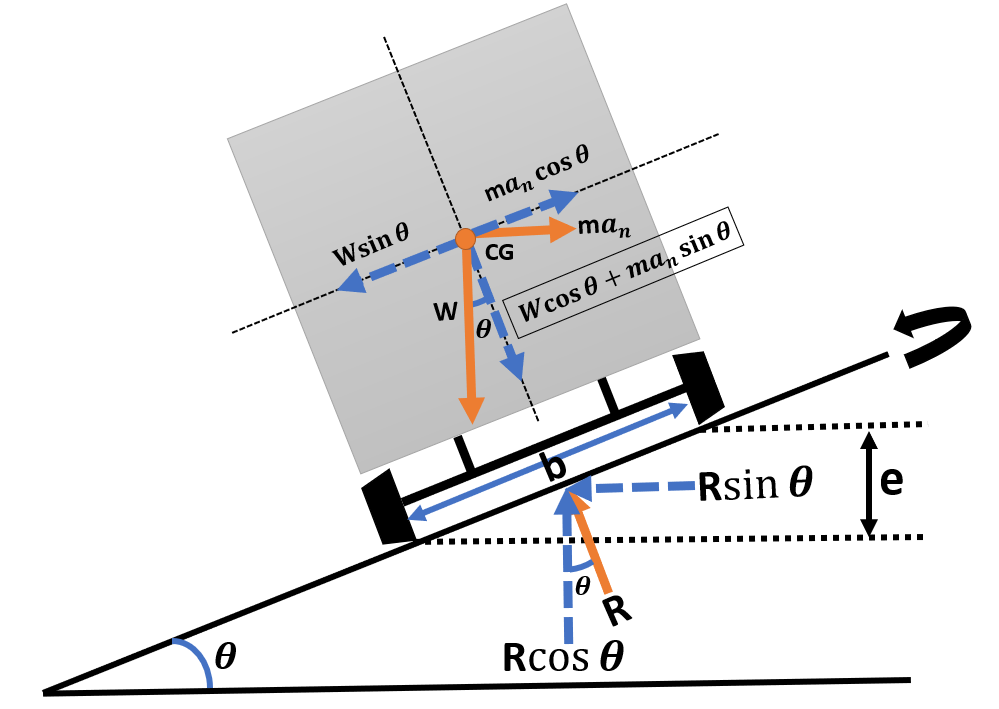
\includegraphics[scale=0.5]{locomotive_banked.png}
	\end{figure}
	\begin{itemize}
		\item In order for the flanges on the rail's wheels to not experience any sideways thrust, the outer rail is raised by a height \textbf{e} compared to the inner rail. This is called \textbf{Super elevation}
		\item From the above diagram, we can infer that $e = b\sin\theta \approx b\tan\theta \implies \boxed{e = \dfrac{bV^2}{gr}}$
	\end{itemize}\hrulefill
%-----------------------------------------------------------------------------------------%
\section{Belt, Rope and Pulley}
\subsection{Flat Belt}
	\begin{itemize}
		\begin{figure}[H]
			\centering
			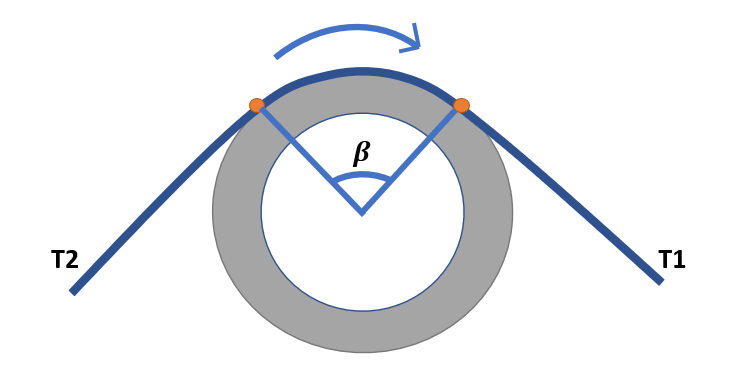
\includegraphics[scale=0.4]{flatbelt.png}
			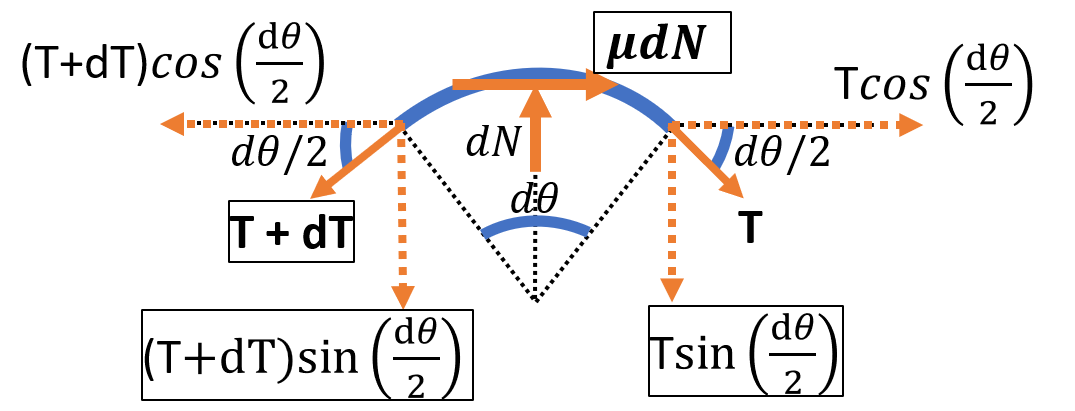
\includegraphics[scale=0.4]{flatbeltelement.png}
		\end{figure}
		\item By $\sum F_x=0 \implies T\cos\dfrac{d\theta}{2}+\mu dN = (T+dT)\cos\dfrac{d\theta}{2} \implies \boxed{\mu dN = dT} \impliedby$ (Here, $\mu dN$ is frictional force)
		\item Similarly By $\sum F_y=0 \implies dN = (T+dT)sin\dfrac{d\theta}{2}+T\sin\dfrac{d\theta}{2} \implies \boxed{dN = Td\theta}$
		\item From the above two results, $\mu Td\theta = dT \implies \mu d\theta = \dfrac{dT}{T} \implies \bigintss_{T_1}^{T_2}\dfrac{dT}{T} = \int_{0}^{\beta}\mu d\theta \implies \ln\left(\dfrac{T_2}{T_1}\right) = \mu\beta$
		\item $\boxed{T_2=T_1e^{\mu\beta}}\impliedby$ ($\beta$ = Total angle of contact \textbf{in Radians})
		\item $T_2$ = Tight side, $T_1$ = Slack side		
		\item \textbf{Always in formula: Tight slide / Slack side}		
		\item If a rope were wrapped around the drum n times, then $\beta=2\pi n$
	\end{itemize}\hrulefill
%-----------------------------------------------------------------------------------------%
\subsection{Rope or V-Belt}
	\begin{itemize}
		\item \fbox{\textbf{DERIVATION REQUIRED $\impliedby \impliedby \impliedby \impliedby \impliedby$}}	
		\item $\boxed{\dfrac{T_2}{T_1}=e^{\left(\dfrac{\mu\beta}{\sin\alpha}\right)}}\impliedby$ (Applicable only when the rope/belt is about to slip)
		\item Where $\alpha$ = groove angle with respect to vertical
	\end{itemize}\hrulefill
%-----------------------------------------------------------------------------------------%
\subsection{Advantages of Rope or V-Belt over Flat belts}
	\begin{itemize}
		\item Rope drives are more suitable for transmitting large powers
		\item In Rope drives, sideways slipping do not occur due to the presence of grooves
	\end{itemize}\hrulefill
%-----------------------------------------------------------------------------------------%
\section{Tension in the Belt}
\subsection{Initial Tension}
	\begin{itemize}
		\item When the belt drive is at rest, some initial tension is always maintained to keep the belt tightly fit on the pulleys. This is called Initial tension ($T_i$)
		\item While transmitting power, the tension becomes $T1=T_i-\delta T$ (slack) and on the other side it becomes $T_2=T_i+\delta T$ (Tight). This change from initial tension is same for both side as the material is assumed to be elastic
		\item $\boxed{T_i=\dfrac{T_1+T_2}{2}}$
	\end{itemize}\hrulefill
%-----------------------------------------------------------------------------------------%
\subsection{Centrifugal Tension}
	\begin{itemize}
		\item While transmitting power, the belt running in a circular path over a pulley, experiences centrifugal force which tends to move the belt away from the contact surface, thereby reducing normal reaction and hence the friction and hence the Transmitting power
		\item In addition to the above, it also induces an extra tension called \textbf{centrifugal tension} on the belt/rope.
		
	\end{itemize}
%-----------------------------------------------------------------------------------------%
\chapter{Work and Energy}
	\begin{itemize}
		\item
	\end{itemize}
%-----------------------------------------------------------------------------------------%
\chapter{Virtual work}
	\begin{itemize}
		\item
	\end{itemize}
%-----------------------------------------------------------------------------------------%
\chapter{Center of Gravity and Moment of Inertia}
	\begin{itemize}
		\item
	\end{itemize}
%-----------------------------------------------------------------------------------------%
\chapter{Impulse and Momentum}
	\begin{itemize}
		\item
	\end{itemize}
%-----------------------------------------------------------------------------------------%
\chapter{Lagrangian Equation}
	\begin{itemize}
		\item
	\end{itemize}
\end{document}
%-----------------------------------------------------------------------------------------%
%-----------------------------------------------------------------------------------------%
%-----------------------------------------------------------------------------------------%
